%%%% ijcai26.tex

\typeout{IJCAI--ECAI 26 Instructions for Authors}

% These are the instructions for authors for IJCAI--ECAI 26.

\documentclass{article}
\pdfpagewidth=8.5in
\pdfpageheight=11in

% The file ijcai26.sty is a copy from ijcai22.sty
% The file ijcai22.sty is NOT the same as previous years'
\usepackage{ijcai26}

% Use the postscript times font!
\usepackage{times}
\usepackage{soul}
\usepackage{url}
\usepackage[hidelinks]{hyperref}
\usepackage[utf8]{inputenc}
\usepackage[small]{caption}
\usepackage{graphicx}
\usepackage{amsmath}
\usepackage{amsthm}
\usepackage{multirow}
\usepackage{threeparttable}
\usepackage{amssymb}
\usepackage{amsfonts}
\usepackage{bm}
\usepackage{booktabs}
\usepackage{algorithm}
\usepackage{algorithmic}
\usepackage{xcolor}
\usepackage[switch]{lineno}

% Comment out this line in the camera-ready submission
\linenumbers

\urlstyle{same}

% the following package is optional:
%\usepackage{latexsym}

% See https://www.overleaf.com/learn/latex/theorems_and_proofs
% for a nice explanation of how to define new theorems, but keep
% in mind that the amsthm package is already included in this
% template and that you must *not* alter the styling.
\newtheorem{example}{Example}
\newtheorem{theorem}{Theorem}

% Following comment is from ijcai97-submit.tex:
% The preparation of these files was supported by Schlumberger Palo Alto
% Research, AT\&T Bell Laboratories, and Morgan Kaufmann Publishers.
% Shirley Jowell, of Morgan Kaufmann Publishers, and Peter F.
% Patel-Schneider, of AT\&T Bell Laboratories collaborated on their
% preparation.

% These instructions can be modified and used in other conferences as long
% as credit to the authors and supporting agencies is retained, this notice
% is not changed, and further modification or reuse is not restricted.
% Neither Shirley Jowell nor Peter F. Patel-Schneider can be listed as
% contacts for providing assistance without their prior permission.

% To use for other conferences, change references to files and the
% conference appropriate and use other authors, contacts, publishers, and
% organizations.
% Also change the deadline and address for returning papers and the length and
% page charge instructions.
% Put where the files are available in the appropriate places.


% PDF Info Is REQUIRED.

% Please leave this \pdfinfo block untouched both for the submission and
% Camera Ready Copy. Do not include Title and Author information in the pdfinfo section
\pdfinfo{
/TemplateVersion (IJCAI.2026.0)
}

\title{IJCAI--ECAI 26 Formatting Instructions}

% Single author syntax
\author{
    Author Name
    \affiliations
    Affiliation
    \emails
    email@example.com
}

% Multiple author syntax (remove the single-author syntax above and the \iffalse ... \fi here)
\iffalse
\author{
First Author$^1$
\and
Second Author$^2$\and
Third Author$^{2,3}$\And
Fourth Author$^4$\\
\affiliations
$^1$First Affiliation\\
$^2$Second Affiliation\\
$^3$Third Affiliation\\
$^4$Fourth Affiliation\\
\emails
\{first, second\}@example.com,
third@other.example.com,
fourth@example.com
}
\fi

\begin{document}

\maketitle

\begin{abstract} 
Multi-task reinforcement learning (MTRL) enables agents to share knowledge across multiple related tasks. 
However, most existing methods suffer from negative transfer because they share parameters at the task level without modeling fine-grained procedural structures. 
These structures, common in robotic tasks like picking and assembling, are often stage-regular and prove essential for transferable skill reuse.
Accordingly, we propose Stage-Masked Policy (SMP), a unified MTRL framework that explicitly exploits procedural structure to enable efficient, scalable multi-task knowledge transfer. 
Specifically SMP comprises three key components: (1) Stage division, which segments tasks into interpretable execution stages; (2) Similarity calculation, which dynamically quantifies behavioral similarity across tasks using high-return trajectories; and (3) Mask-based policy activation which enables selective parameter sharing among multiple tasks based on their stage similarities.
As a result, SMP enables fine-grained knowledge transfer, mitigates negative transfer, and facilitates learning in sparse-reward, aspects often overlooked in prior work.
Empirical results on the Meta-World benchmark demonstrate that SMP significantly outperforms multiple baselines, both on convergence rate and asymptotic performance.
Particularly in MT-10, SMP outperforms prior methods by over 20\% under sparse-reward settings and achieves 10\% higher success rate in dense-reward scenarios, and learns the task faster in the few-shot scenario. 
\end{abstract}

\section{Introduction}

\begin{figure}[htbp]
   \centering
        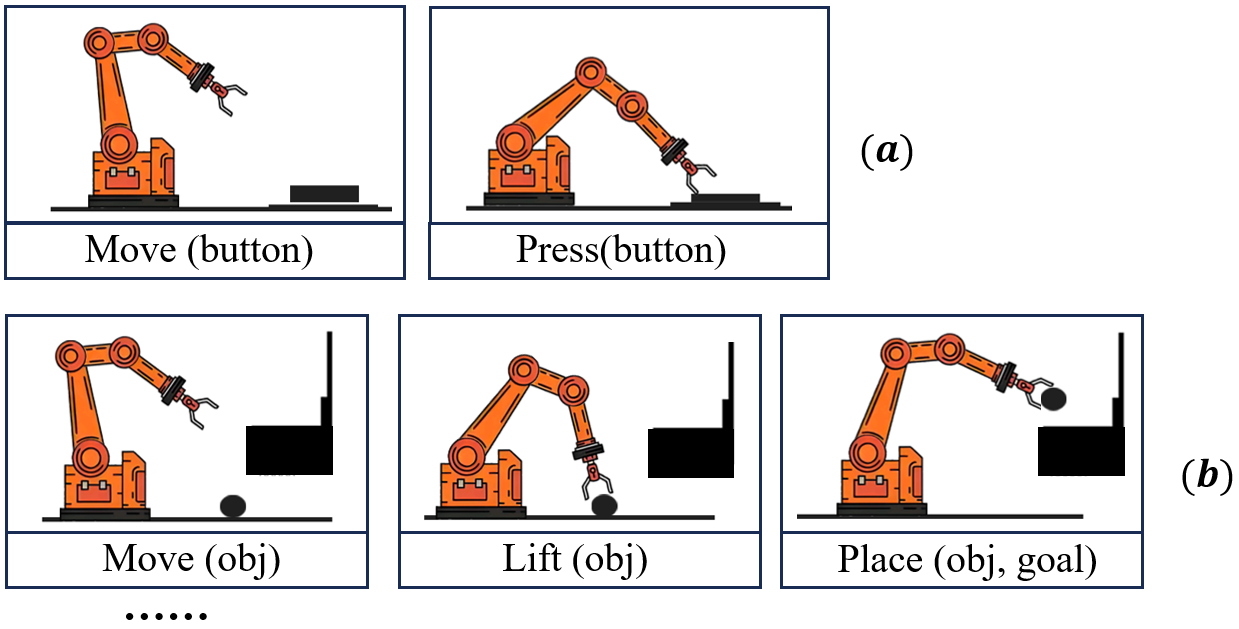
\includegraphics[width=0.48\textwidth]{F-1-1.PNG} 
\caption{Illustration of a robotic arm and its 2 tasks: (\textit{a}) \textsc{Press-Down}, (\textit{b}) \textsc{Pick-and-Put}. The tasks are staged, and there are intercorrelations between the stages from different tasks.}
\label{fig:task_sim}
\end{figure}

%MTRL 背景与应用
%\textcolor{blue}{1. Multi-task reinforcement learning (MTRL) is useful. MTRL Background and Applications}

Multi-task reinforcement learning (MTRL) aims to learn a single generalized policy for multiple tasks by leveraging shared representations and experiences \cite{q2, q60}. 
In practical applications, such as a robotic arm handling various distinct operations, MTRL has been shown to effectively enhance data utilization and promote knowledge transfer across interrelated tasks \cite{q7}. 
However, standard MTRL generally assumes a fixed, predefined set of tasks. In realistic, open-ended environments, agents are increasingly required to incrementally acquire new skills over their lifespan without losing prior capabilities \cite{q16,q84}. 
Consequently, there is a natural demand to extend MTRL into a continual learning setting, where the primary objective is to sequentially adapt to novel tasks while maintaining high proficiency and parameter efficiency ~\cite{q11}.

%\textcolor{blue}{The core challenges and the need to XXX. Why?}
%核心挑战
Realizing such continual MTRL agents, however, is fundamentally bottlenecked by the stability-plasticity dilemma and severe inter-task interference. 
When a monolithic network adapts to a novel task, traditional optimization intrinsically modifies the shared weights to absorb new representations. 
As evidenced by recent studies on continual learning \cite{q19,q20}, such destructive updates inevitably overwrite previously established skills, leading to catastrophic forgetting. 
Conversely, attempting to rigidly protect these weights (e.g., via simple regularization) drastically limits the model's capacity to learn new tasks \cite{q14}. 
Since network capacity and knowledge retention are inherently linked, weight-modifying adaptation is unsustainable for lifelong skill accumulation. 
\emph{A core challenge is thus to develop mechanisms that can efficiently resolve gradient conflicts among existing tasks while adapting to new environments without altering the foundational knowledge base.}


%现有 MTRL 方法回顾
%\textcolor{blue}{2. Review of existing MTRL methods.}
Numerous approaches have been proposed to mitigate these interferences, yet they typically focus on isolated aspects of the dilemma. 
For instance, PopArt \cite{q12} aligns reward scales across tasks while sharing the entire backbone. 
To provide finer-grained control, modular architectures like Soft.M \cite{q51} and PaCo \cite{q36} employ soft routing or compositional masks for parameter sharing.
While highly effective in static MTRL, these approaches rely on continuous weight modifications, leaving them vulnerable to catastrophic forgetting in sequential task streams. 
Alternatively, gradient surgery techniques, such as PCGrad \cite{i14}, explicitly resolve task conflicts by projecting interfering gradients onto orthogonal planes. Nevertheless, this projection can induce gradient norm reduction that slows convergence, and it lacks mechanisms to safeguard prior knowledge against future updates. 
To address gradient conflict issues, additional architectures such as Projection Task-Specific Layers (PTSL)\cite{q43} share a backbone and add task-specific modules.
While this reduces gradient conflicts, it leads to linear parameter scaling and suffers from the "structural cold start" problem, while still struggling to handle catastrophic forgetting because the agent must be randomly initialized and trained from scratch for each new task.


%为什么使用0/1掩码作为基础架构，为什么考虑相似性，怎么实现连续学习。为什么需要表示(其他人做法，预实验，为什么使用VAE),为什么需要基于梯度的剪枝策略(软模块，梯度)
Recent advances in continual learning have investigated the use of parameter isolation to mitigate interference.
For instance, Piggyback \cite{i13} demonstrated that learning task-specific binary masks over a frozen backbone effectively prevents forgetting.
While this method strictly preserves prior knowledge, it faces a severe "structural cold-start" problem: finding an optimal sparse sub-network for each new task from scratch is highly sample-inefficient in RL.
Fortunately, the Lottery Ticket Hypothesis (LTH) \cite{n1} offers a promising theoretical perspective.
Studies have empirically verified that sparse functional sub-networks robustly exist even under the non-stationary reward signals of RL \cite{n2}.
More crucially, the topological structures of these sparse sub-networks encode generic inductive biases that are transferable across similar tasks \cite{n3}.
To the best of our knowledge, \emph{no prior work has systematically exploited latent task similarities to guide dynamic mask evolution in continual MTRL}.

%预实验结果，初步验证问题假设
To empirically illustrate the limitations of current MTRL architectures in continuous adaptation, we conducted a set of preliminary experiments.
We assessed the zero-to-few-shot adaptation performance of major MTRL approaches by introducing two previously unseen tasks (\textit{drawer-open} and \textit{window-open}) to a pre-trained backbone.
The results show that state-of-the-art dense-sharing and soft-routing methods (e.g., MT-SAC, Soft.M, CARE) completely fail to adapt, stagnating at near-zero success rates within 300 episodes.
Even PTSL, which appends new adapter layers to mitigate forgetting, fails due to the structural cold-start problem.
Interestingly, a vanilla dynamic masking approach (an un-frozen ablation of our framework) achieves a 31.6\% success rate on a simpler new task, but still struggles with harder tasks (2.3\%) due to the vast topological search space.
Furthermore, leaving the backbone un-frozen inevitably disrupts prior knowledge.
\emph{A key insight from this preliminary study is that while masking provides a viable pathway for task isolation, naively searching for masks in an un-frozen network is highly sample-inefficient and still vulnerable to forgetting.}


%基于前面的问题，说明解释对应解决方案核心方法：核心模块是两个，一个是伪0/1掩码和基于混合梯度评分的掩码更新模块（包括基于混合梯度更新的自更新和基于相似性的跨任务更新），另外一个是基于状态-动作序列的相似性评估模块。
Driven by the structural priors of the Lottery Ticket Hypothesis \cite{n1}, our method focuses on two core modules:
(1) Latent Similarity Evaluation, which encodes state-action sequences via a Task-VAE to explicitly quantify behavioral alignment across tasks in a latent space;
(2) Conflict-Aware Masked Policy, which employs pseudo-binary masks to selectively activate reusable sub-networks, optimized dynamically through intra-task self-updates (via hybrid gradient scoring) and cross-task transfer (via latent similarity).
By decoupling structural search from weight optimization, DPTE reduces the severe interference among heterogeneous tasks and enables robust, collision-free knowledge transfer.
This approach substantiates our insight: effective continual MTRL is possible when adaptation is conducted via topological evolution rather than weight modification.


%总结创新&贡献
We evaluate DPTE on the Meta-World MT10 and MT50 benchmarks \cite{q15} under continual learning settings. 
Experiments show that DPTE improves convergence speed and prevents catastrophic forgetting, especially in sequential task scenarios. 
Combined results from multi-task co-learning and few-shot adaptation experiments further indicate its potential for real-world deployment.
Our main contributions are summarized as follows:
\begin{itemize}
\item We systematically demonstrate that parameter isolation via topological structures is crucial for continual MTRL, especially under sequential task extensions.
\item Building upon the structural priors of the Lottery Ticket Hypothesis, we propose a novel framework featuring latent similarity evaluation and conflict-aware masked policy to enable zero-interference co-learning and frozen-backbone adaptation.
\item We evaluate DPTE across multi-task co-learning and continual few-shot setups, achieving rapid topological warm-starts and consistently surpassing state-of-the-art baselines.
\end{itemize}



\section{Related Work}

% 1. MTRL与优化干扰 (保留对梯度手术的分析，引出拓扑隔离的必要性)
MTRL aims to distill a generalized policy across interrelated tasks but frequently suffers from severe optimization interference (negative transfer). 
Existing solutions primarily focus on gradient surgery or soft architectural routing. 
Gradient surgery methods, such as PCGrad \cite{i14}, attempt to resolve task conflicts mathematically by projecting interfering gradients. However, these projections often induce gradient norm reduction, slowing down convergence. 
Alternatively, routing methods like Soft.M \cite{q51} and PaCo \cite{q36} use soft modularization for parameter sharing. 
Recently, Projected Task-Specific Layers (PTSL) \cite{q43} allocates independent network subspaces for each task via projection matrices. 
While alleviating interference in static co-learning environments, these methods rely on dense weight modifications or static structural allocations. 
When applied to continual learning, they struggle to simultaneously decouple conflicting gradients and prevent catastrophic forgetting without destroying prior representations.


%连续学习相关研究
%% 2. 连续学习中我们为什么使用掩码和网络拓扑作为主要研究方向，比如LoRA 的局限性 (“权重空间”)
To address catastrophic forgetting in sequential task extensions, recent advances have explored Parameter-Efficient Fine-Tuning (PEFT) and representation transfer. 
Methods like QueST \cite{n4} extract reusable latent skill abstractions for continuous control but do not explicitly isolate the underlying network parameters, risking interference during sequential updates. 
Alternatively, additive modules have been widely adopted. 
For instance, recent embodied continual frameworks like Task-aware MoILE \cite{n5} employ incremental LoRA experts to adapt to new tasks while preserving prior knowledge. 
Although highly parameter-efficient, these additive approaches operate primarily in the weight space (e.g., adding low-rank updates $\Delta W$). 
They do not alter the fundamental routing topology of the backbone. Consequently, they cannot physically decouple the interfering gradient flows when multiple tasks interact, nor can they efficiently transfer structural priors to overcome the cold-start problem in novel RL environments.


% 3. 彩票假设与拓扑隔离 (祭出我们的理论：掩码在拓扑空间的作用)

To simultaneously resolve gradient conflicts and structural cold-start, we pivot from weight-space adaptation to topological isolation. 
LTH \cite{n1} provides the theoretical bedrock for this approach, positing that dense networks contain sparse sub-networks ("winning tickets") capable of matching full-model performance. 
Recent studies verify that such sparse sub-networks robustly exist in RL \cite{n2} and encode generic inductive biases transferable across similar tasks \cite{n3}. 
Unlike low-rank weight updates, learning binary masks acts directly in the \emph{topological space}, physically severing conflicting gradient pathways during multi-task co-learning. 
Our DPTE framework fully exploits this property. By measuring latent task similarities to guide dynamic mask evolution, DPTE inherits transferable topological priors. 
This approach elegantly unifies zero-interference co-learning and frozen-backbone continual adaptation through pure structural evolution.


\begin{table}[h]
\centering
\resizebox{\columnwidth}{!}{%
\begin{tabular}{@{}lccc@{}}
\toprule
\textbf{Method} & \textbf{Param. Isol.} & \textbf{Frozen Back.} & \textbf{Struct. Trans.} \\
\midrule
MT-SAC \cite{q15}  & $\times$ & $\times$ & $\times$ \\
CARE \cite{q69}    & $\times$ & $\times$ & $\times$ \\
Soft.M \cite{q51}  & $\checkmark$ & $\times$ & $\times$ \\
PaCo \cite{q36}    & $\checkmark$ & $\times$ & $\times$ \\
PTSL \cite{q43}    & $\checkmark$ & $\checkmark$ & $\times$ \\
\textbf{SMP (Ours)}& $\checkmark$ & $\checkmark$ & $\checkmark$ \\
\bottomrule
\end{tabular}%
}
\caption{Comparison of evaluated architectures. SMP uniquely achieves strict parameter isolation and continual knowledge preservation while enabling rapid adaptation via structural transfer.}
\label{tab:comparison}
\end{table}


\section{Preliminaries}

\paragraph{Continual Multi-Task Reinforcement Learning.} 
We formulate each task $T^{(i)}$ as a Markov Decision Process (MDP), defined by a tuple $\mathcal{M}^{(i)} = \langle \mathcal{S}, \mathcal{A}, \mathcal{P}^{(i)}, \mathcal{R}^{(i)}, \gamma \rangle$. 
The agent experiences a dual-phase lifecycle. 
During the \emph{co-learning phase}, the agent is exposed to a base set of $N$ tasks, $\mathcal{T}_{base} = \{T^{(1)}, \dots, T^{(N)}\}$. 
The objective is to learn a parameterized policy $\pi_{\bm{\theta}}$ that minimizes the average expected loss (i.e., negative return) across all base tasks: $\mathcal{L}_{base}(\bm{\theta}) = \frac{1}{N} \sum_{i=1}^{N} \mathcal{L}_i(\bm{\theta})$.
During the \emph{continual adaptation phase}, a sequence of novel tasks $\mathcal{T}_{novel} = \{T^{(N+1)}, T^{(N+2)}, \dots\}$ arrives incrementally. 
Upon the arrival of $T^{(k)}$, the agent must rapidly adapt to minimize $\mathcal{L}_k(\bm{\theta})$ without causing catastrophic forgetting on previously learned tasks.

\paragraph{Gradient Conflict in Dense Networks.} 
In standard MTRL, the policy is parameterized by a monolithic dense weight vector $\bm{\theta} \in \mathbb{R}^d$. 
Let $\bm{g}_i = \nabla_{\bm{\theta}} \mathcal{L}_i(\bm{\theta})$ denote the task-specific gradient. 
As formally identified by optimization studies \cite{i14}, \emph{gradient conflict} occurs when the optimization directions of two heterogeneous tasks diverge. Mathematically, a conflict arises when:
\begin{equation}
\bm{g}_i^\top \bm{g}_j < 0 \quad \text{for } i \neq j.
\label{eq:gradient_conflict}
\end{equation}
When Eq.~\ref{eq:gradient_conflict} holds, moving $\bm{\theta}$ in the direction of $-\bm{g}_i$ intrinsically increases the loss of task $j$, leading to severe negative transfer and preventing convergence to a joint optimum.

\paragraph{Topological Decoupling via Lottery Ticket Hypothesis.} 
To explicitly resolve gradient conflicts during co-learning and theoretically guarantee zero forgetting during continual adaptation, we reformulate the optimization space through the lens of the Lottery Ticket Hypothesis (LTH) \cite{n1}. 
Instead of relying solely on the dense continuous weights $\bm{\theta}$, we decouple the policy parameterization into a shared continuous backbone $\bm{\theta} \in \mathbb{R}^d$ and a set of task-specific binary masks $\bm{m}^{(i)} \in \{0, 1\}^d$. The effective parameters for task $i$ become $\bm{\phi}^{(i)} = \bm{\theta} \odot \bm{m}^{(i)}$, and the policy is parameterized as $\pi(a | s; \bm{\phi}^{(i)})$.

This topological formulation fundamentally alters the gradient flow. During the \emph{co-learning phase}, the agent \textbf{jointly optimizes} both the shared weights $\bm{\theta}$ and the topological masks $\bm{m}^{(i)}$. Let $\tilde{\bm{g}}_i = \nabla_{\bm{\phi}^{(i)}} \mathcal{L}_i$ denote the raw gradient with respect to the active sub-network. By applying the chain rule, the effective gradient propagated to the shared backbone becomes $\hat{\bm{g}}_i = \nabla_{\bm{\theta}} \mathcal{L}_i = \tilde{\bm{g}}_i \odot \bm{m}^{(i)}$. Consequently, the inner product between two task gradients on the shared backbone is reformulated as:
\begin{equation}
\hat{\bm{g}}_i^\top \hat{\bm{g}}_j = \sum_{k=1}^{d} \tilde{g}_{i,k} \tilde{g}_{j,k} \underbrace{m_k^{(i)} m_k^{(j)}}_{\text{Topological Gating}}.
\label{eq:masked_gradient}
\end{equation}
Eq.~\ref{eq:masked_gradient} reveals a critical theoretical insight: by dynamically evolving the masks to be mutually exclusive ($m_k^{(i)} m_k^{(j)} = 0$) at specific dimensions $k$ where the raw gradients conflict ($\tilde{g}_{i,k} \tilde{g}_{j,k} < 0$), the network can physically decouple the optimization pathways. This mathematically ensures $\hat{\bm{g}}_i^\top \hat{\bm{g}}_j \ge 0$, eliminating negative transfer while maintaining parameter sharing for aligned gradients.

During the subsequent \emph{continual adaptation phase}, the fully optimized backbone $\bm{\theta}^*$ acts as a dense repository of generic structural priors (i.e., a pool of winning tickets). For any novel task $T^{(k)}$, $\bm{\theta}^*$ is strictly frozen ($\Delta \bm{\theta}^* = 0$), and the agent transitions to a \textbf{purely structural search} for the optimal mask $\bm{m}^{(k)}$. This frozen-backbone constraint renders catastrophic overwriting mathematically impossible, perfectly resolving the stability-plasticity dilemma.

\section{Methodology}


\begin{figure*}[!htp]
\centering
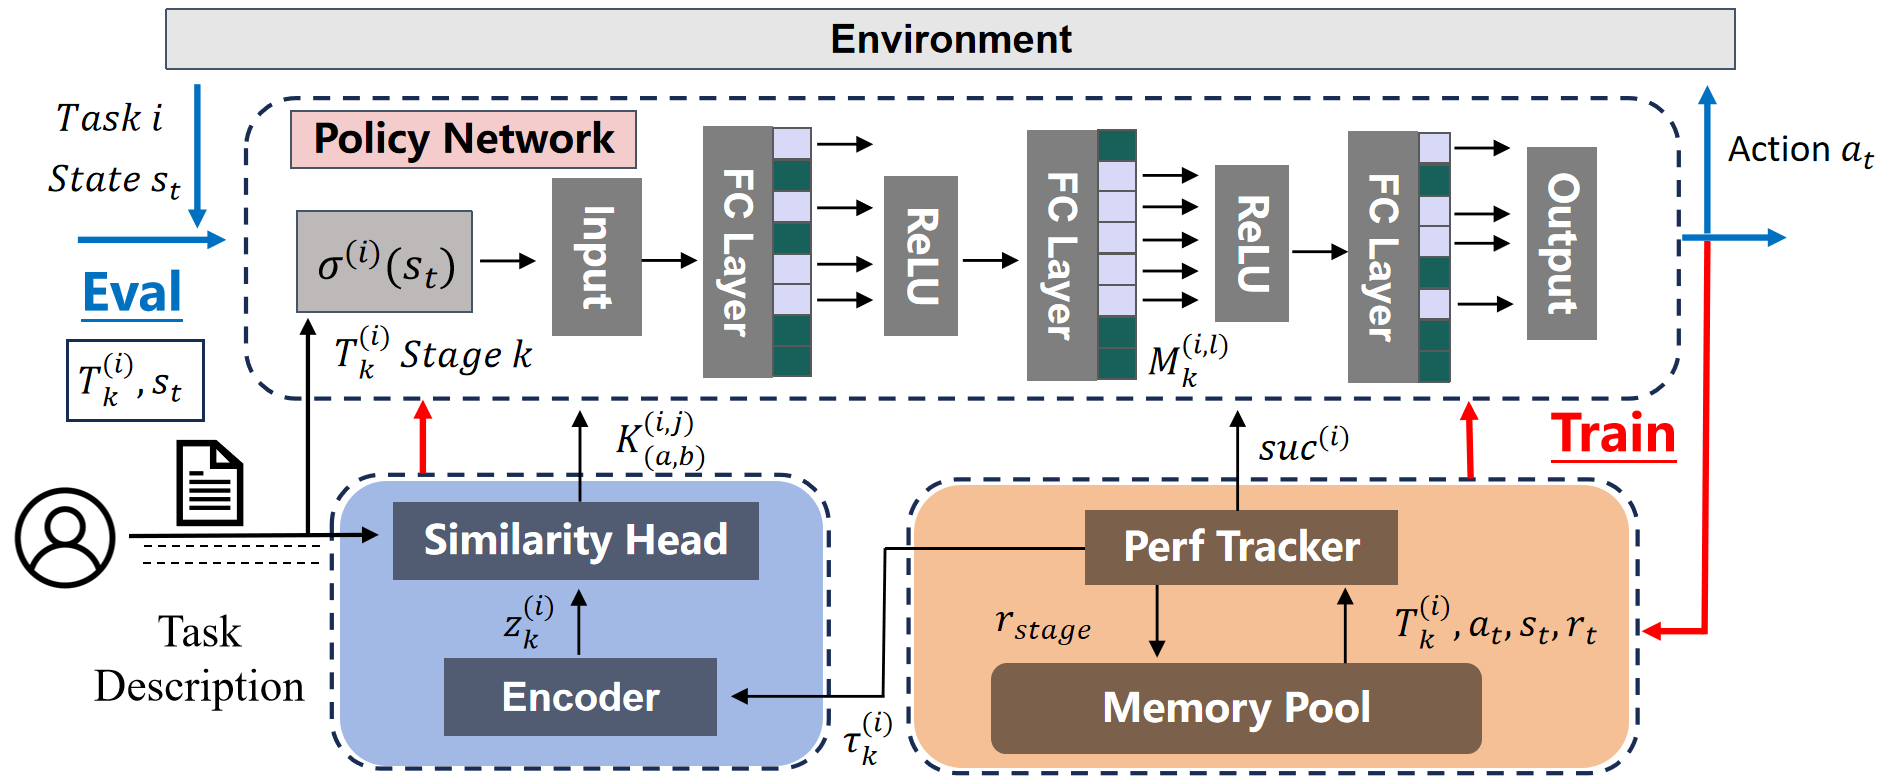
\includegraphics[width=16cm,height=6cm]{F-3.PNG}\\
\caption{
The overall framework of Dual-Phase Topological Evolution (DPTE). 
(1) During Co-learning, the Conflict-Aware Masked Policy dynamically decouples interfering gradients via topological gating. 
(2) During Continual Adaptation, the Latent Similarity Engine guides the transfer of mask priors to a frozen backbone, enabling zero-forgetting adaptation.
}
\label{fig:fig_3}
\end{figure*}

Fig.\,\ref{fig:fig_3} illustrates our proposed Dual-Phase Topological Evolution (DPTE) framework. 


\renewcommand{\algorithmicrequire}{\textbf{Input:}}
\renewcommand{\algorithmicensure}{\textbf{Output:}}
\begin{algorithm}[t]
\caption{Dual-Phase Topological Evolution (DPTE)}
\label{alg:dpte}
\begin{algorithmic}[1]
\REQUIRE Base tasks $\mathcal{T}_{base}$, Novel task stream $\mathcal{T}_{novel}$
\ENSURE Optimized backbone $\bm{\theta}^*$, Task-specific masks $\{\bm{m}^{(i)}\}$

\STATE \textcolor{gray}{\% Phase 1: Conflict-Aware Masked Co-learning}
\WHILE{not converged on $\mathcal{T}_{base}$}
    \STATE Update Task-VAE and compute similarity matrix $\mathcal{K}$ via Eq.~\ref{eq:similarity}
    \FOR{each base task $i \in \mathcal{T}_{base}$}
        \STATE Compute raw gradient $\bm{g}_i$ w.r.t masked weights $\bm{\theta} \odot \bm{m}^{(i)}$
        \STATE \textbf{Conflict Resolution:} If $g_{i,k} g_{j,k} < 0$, force $m_k^{(i)} m_k^{(j)} = 0$ 
    \ENDFOR
    \STATE Update shared backbone $\bm{\theta}$ using physically decoupled gradients
\ENDWHILE
\STATE Save and freeze optimized backbone: $\bm{\theta}^* \leftarrow \bm{\theta}$

\STATE 
\STATE \textcolor{gray}{\% Phase 2: Frozen-Backbone Continual Adaptation}
\FOR{each novel task $T^{(k)} \in \mathcal{T}_{novel}$}
    \STATE Find most similar base task via VAE: $j^* = \arg\max_j \mathcal{K}(k, j)$
    \STATE \textbf{Topological Warm-start:} Initialize mask $\bm{m}^{(k)} \leftarrow \bm{m}^{(j^*)}$
    \WHILE{not converged on $T^{(k)}$}
        \STATE Optimize \emph{only} mask $\bm{m}^{(k)}$ with frozen backbone ($\Delta \bm{\theta}^* = 0$)
    \ENDWHILE
\ENDFOR

\RETURN $\bm{\theta}^*$, $\{\bm{m}^{(i)}\}$
\end{algorithmic}
\end{algorithm}


\subsection{Overall Framework}
%不用讲具体方法只讲输入/输出和在整体框架中的作用即可。

DPTE augments the conventional monolithic parameter-sharing paradigm by shifting the locus of optimization from dense weight modification to explicit topological routing. 
It comprises two tightly coupled core modules that function cyclically, playing distinct roles across the dual-phase lifecycle to enable fine-grained, conflict-free knowledge transfer:

% 模块 1：潜变量相似性引擎
\textbf{1. Latent Similarity Engine (Task-VAE)}
To determine what structural knowledge to share or transfer across tasks, this module explicitly quantifies the behavioral equivalence between different tasks in a latent space.
\begin{itemize}
\item \textbf{Input/Output:} Taking task-specific state-action trajectories $\tau^{(i)}$ as input, it encodes them into geometry-invariant latent distributions $\bm{z}^{(i)}$ via a Task-VAE $E_\phi$, and outputs a pairwise similarity matrix $\mathcal{K}$:
\begin{equation}
\mathcal{K}(i,j) = \text{SIM}(\bm{z}^{(i)} \| \bm{z}^{(j)}), \quad \text{where } \bm{z} \sim E_{\phi}(\tau).
\label{eq:similarity}
\end{equation}
\item \textbf{Role in Co-learning Phase:} It identifies behavioral alignments among base tasks, guiding the initial mask evolution to share parameters among highly correlated tasks, thereby accelerating joint convergence.
\item \textbf{Role in Adaptation Phase:} The matrix $\mathcal{K}$ serves as a topological transfer map. Upon the arrival of a novel task, it guides the policy to inherit the binary mask from the most behaviorally similar prior task, providing a structural warm-start that overcomes sample inefficiency.
\end{itemize}

% 模块 2：冲突感知掩码策略
\textbf{2. Conflict-Aware Masked Policy}
Finally, the agent executes actions using a shared backbone modulated by dynamic topological masks.
\begin{itemize}
\item \textbf{Input/Output:} Conditioned on the state $s_t$, the task index $i$, and the similarity guidance $\mathcal{K}$, the policy activates a task-specific pseudo-binary mask $\bm{m}^{(i)}$. The action $a_t$ is generated by the masked effective parameters:
\begin{equation}
a_t \sim \pi(a_t | s_t; \bm{\theta} \odot \bm{m}^{(i)}).
\label{eq:policy_execution}
\end{equation}
\item \textbf{Role in Co-learning Phase:} This mechanism acts as a dynamic gradient decoupler. Driven by a hybrid gradient scoring mechanism, it physically isolates parameter dimensions (i.e., forcing $m_k^{(i)} m_k^{(j)} = 0$) where raw gradients conflict, explicitly eliminating negative transfer.
\item \textbf{Role in Adaptation Phase:} It acts as a strict knowledge preserver. By freezing the shared backbone ($\Delta \bm{\theta} = 0$) and relying solely on the optimization of the new mask $\bm{m}^{(k)}$, it mathematically guarantees zero catastrophic forgetting of prior skills.
\end{itemize}

\subsection{Phase 1: Conflict-Aware Masked Co-learning}

Given the theoretical formulation defined in Section 3, we implement the Conflict-Aware Masked Policy as a dynamic, gradient-guided gating mechanism.
Its primary role is to dynamically route the optimization trajectories in the topological space, which subsequently eliminates negative transfer during the joint training of the base task set $\mathcal{T}_{base}$.


As formalized in Phase 1 of Algorithm~\ref{alg:dpte}, the module operates online by evaluating the task-specific raw gradients $\bm{g}_i = \nabla_{\bm{\phi}^{(i)}} \mathcal{L}_i$ at each optimization step. 
To physically resolve the gradient conflict defined in Eq.~\ref{eq:gradient_conflict}, we introduce a \emph{hybrid gradient scoring} mechanism.
Specifically, the topological gating follows a competitive routing logic:
\begin{equation}
m_k^{(i)} = 
\begin{cases} 
0, & \exists j \neq i \text{ s.t. } g_{i,k} g_{j,k} < 0 \text{ and } \mathcal{S}_{j,k} > \mathcal{S}_{i,k} \\ 
1, & \text{otherwise} 
\end{cases}
\label{eq:mask_routing}
\end{equation}
where $\mathcal{S}_{i,k} = |g_{i,k}|$ denotes the priority score, representing the optimization demand of task $i$ on the $k$-th parameter dimension.


A parameter dimension $k$ is exclusively assigned to task $i$ if a gradient conflict occurs and task $i$ exhibits a stronger optimization demand. 
This competitive evaluation ensures that conflicting updates are physically decoupled, mathematically guaranteeing $\hat{\bm{g}}_i^\top \hat{\bm{g}}_j \ge 0$. 
By continuously monitoring the gradient directions and magnitudes, this mechanism provides a collision-free co-learning environment while maximizing positive parameter sharing among aligned tasks.

\subsection{Phase 2: Similarity-Guided Continual Adaptation}

Given the fully optimized shared backbone $\bm{\theta}^*$ established in Phase 1, we implement the Latent Similarity Engine coupled with a frozen-backbone adaptation strategy.
Its primary role is to rapidly assimilate novel tasks from the stream $\mathcal{T}_{novel}$ into the topological space, which subsequently completely prevents catastrophic forgetting and overcomes the structural cold-start bottleneck.

As formalized in Phase 2 of Algorithm~\ref{alg:dpte}, the module operates sequentially upon the arrival of a novel task $T^{(k)}$. 
To theoretically guarantee zero forgetting, we explicitly freeze the continuous dense weights ($\Delta \bm{\theta}^* = 0$). To overcome the sample-inefficient search from scratch, we introduce a \emph{topological warm-start} mechanism guided by latent behavioral similarities. 
Specifically, the mask adaptation follows a similarity-inherited optimization logic:
\begin{equation}
\bm{m}^{(k)} = \arg\min_{\bm{m} \in \{0, 1\}^d} \mathcal{L}_k \left( \bm{\theta}^* \odot \bm{m} \right), 
\label{eq:mask_adaptation}
\end{equation}
\begin{equation*}
\quad \text{initialized via } \bm{m}^{(k)} \leftarrow \bm{m}^{(j^*)}
\end{equation*}
where $j^* = \arg\max_j \mathcal{K}(k, j)$ denotes the most behaviorally aligned prior task. This alignment is explicitly quantified by the Task-VAE similarity engine: $\mathcal{K}(k,j) = \text{SIM}(E_\phi(\tau^{(k)}) \| E_\phi(\tau^{(j)}))$, measuring the geometric distance of trajectory distributions in the latent space.

The continual adaptation process is exclusively restricted to the evolution of the task-specific mask $\bm{m}^{(k)}$ over the frozen structural priors. 
This strict topological restriction ensures that the effective parameters of all prior tasks ($\bm{\theta}^* \odot \bm{m}^{(<k)}$) remain mathematically invariant, explicitly rendering catastrophic overwriting impossible. 
By inheriting the topological winning tickets from similar tasks rather than randomly initializing them, this mechanism effectively bypasses the vast combinatorial search space, providing rapid, zero-interference few-shot adaptation in lifelong learning scenarios.

\subsection{Predicate-based Structured Stage Division}


%在这里只讲“怎么用”，结合 Algorithm 1，重点描述运行时的逻辑
Given the symbolic priors defined in Section 3, we implement the stage division function $\sigma^{(i)}$ as a deterministic, real-time gating mechanism.
Its primary role is to dynamically map the continuous state stream $s_t$ into a discrete stage index $k_t$, which subsequently triggers the stage-specific encoder and policy modules.

As formalized in Algorithm~\ref{alg:stage_id}, the function $\sigma^{(i)}$ evaluates the task progress at each timestep.
Our module operates online by checking the sequence of stage conditions $\{\mathcal{C}_k\}_{k=1}^n$ derived from $\mathbb{P}$.
Specifically, the logical flow follows a waterfall mechanism:
\begin{equation}
k_t = \min\{ k \mid \mathcal{C}_k(s_t; \mathbb{E}) = 0 \}
\end{equation}
The agent is considered to be in stage $k$ if all preceding conditions $\mathcal{C}_{1 \dots k-1}$ are satisfied, but $\mathcal{C}_k$ is not.
This sequential evaluation ensures that the agent strictly follows the procedural hierarchy of the task.
By continuously monitoring the geometric relations between entities , it provides stable structural indices.
%为了利用任务结构先验，我们使用前面提到的谓词逻辑来阶段划分。




\subsection{Encoder and Similarity Calculation}

%解释为什么光有谓词不够，必须要有基于数据的表示。结合Intro,衔接上面的工作，确保逻辑通顺。（提出问题，回答问题）
\paragraph{Motivation.}
While the predicate-based division (Section 4.2) provides discrete structural indices, it does not quantify the kinematic heterogeneity across tasks.
As demonstrated in our Introduction (Figure 2), merely sharing parameters based on semantic labels is insufficient due to diverse physical dynamics and geometric shifts.
Therefore, effective transfer requires a representation that is both functionally distinct and geometrically invariant.
%逻辑链：结构有了-但物理细节缺失-且存在几何干扰-需要新表示。

%基于数据，基于什么数据？定义输入数据。高奖励序列
We adopt a data-driven approach to capture stage-specific dynamics.
Using the indices $k_t$ from the Stage Division Function, we define a Stage Trajectory $\tau^{(i)}_{k}$ as a sequence of state-action pairs $\{(s_t, a_t)\}_{t=1}^{L}$.
To ensure the representation encodes optimal behaviors rather than exploration noise, we maintain a prioritized buffer that stores only high-return trajectories satisfying a length threshold $L_{\min}$.
%逻辑链：为了学表示 - 收集高分轨迹-输入进 EGNN-CVAE 模型。同时能详细解释这个模块的输入

\begin{figure}[htbp]
   \centering
        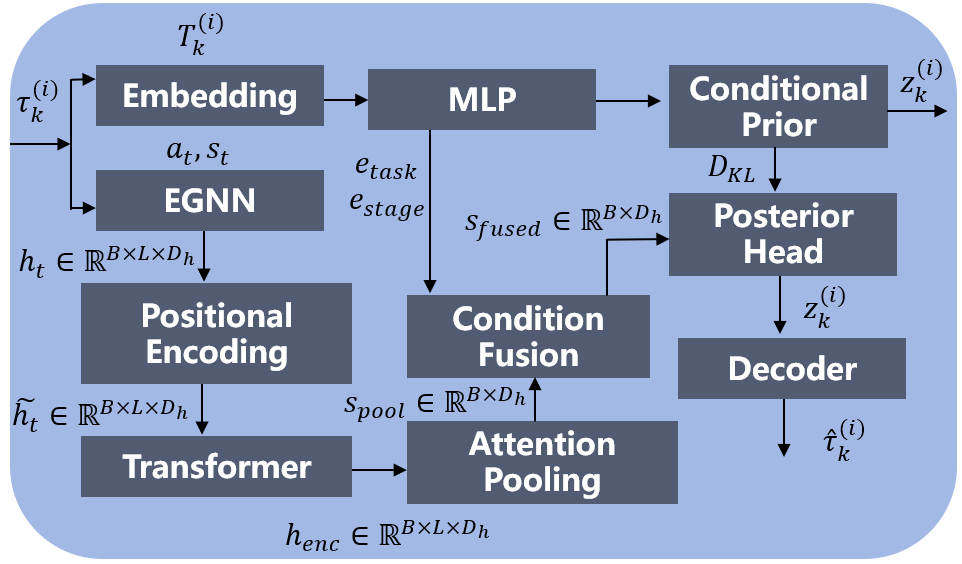
\includegraphics[width=0.48\textwidth]{E-2.png} 
\caption{Architecture of the EGNN-CVAE Encoder. It utilizes an SE(3)-invariant graph frontend to extract geometric features, followed by a Transformer for temporal aggregation, producing a latent distribution $z$ robust to spatial transformations.}
\label{fig:encoder}
\end{figure}


%怎么利用数据。介绍创新部分；给出框架&创新。%怎么利用数据。
\paragraph{Conditioned SE(3)-Invariant Frontend.}
A key challenge in trajectory modeling is the misalignment between spatial geometry and semantic intent. 
Conventional encoders often lack $SE(3)$-invariance, meaning they perceive the same physical action as distinct tasks when subjected to rotations or translations. 
To overcome this. As shown in Figure~\ref{fig:encoder}, we design a Conditioned SE(3) Frontend that integrates EGNN-based message passing with gating. 
At each time step $t$, the module constructs a fully connected graph among entities (e.g., hand, object, goal) and updates node embeddings using relative coordinates, ensuring global frame invariance:
\begin{equation*}
\mathbf{h}_t = \mathrm{EGNN}(s_t, a_t).
\end{equation*}


We add sinusoidal positional encodings to preserve temporal order:
\begin{equation*}
\tilde{\mathbf{h}}_t = \mathrm{PE}(\mathbf{h}_t).
\end{equation*}

%方法流程，方法&组件流水账，但是必须讲解清晰，不能随便给出新的定义
\paragraph{Encoder $E_{\phi}$ Pipeline.}
The encoder comprises three stages capturing both spatial and temporal dependencies:

\begin{enumerate}
    \item Invariant Feature Extraction: The SE(3) Frontend outputs geometry-invariant node features $\mathbf{h}_t$, enhanced with positional encodings $\tilde{\mathbf{h}}_t$ to retain temporal structure.
    
    \item Temporal Aggregation: A multi-layer Transformer encoder processes $\tilde{\mathbf{h}}_{1:L}$ to capture long-range spatiotemporal correlations. 
    An attention pooling layer aggregates the sequence into a global stage descriptor:
    \begin{equation*}
    \mathbf{s}_{\mathrm{pool}} = \mathrm{AttnPool}\!\left(\mathrm{Transformer}\!\left([\tilde{\mathbf{h}}_1, \ldots, \tilde{\mathbf{h}}_L]\right)\right).
    \end{equation*}

    \item Enhanced Conditional Projection: To fuse trajectory semantics with contextual information, we employ an Enhanced Residual Gated Block instead of simple concatenation. 
    Given the condition vector $\mathbf{c}$ (the concatenation of task and stage embeddings), we compute:
    \begin{equation*}
    \mu, \log\sigma^2 = \mathrm{MLP}\!\left(\mathrm{LayerNorm}\!\big(\mathbf{s}_{\mathrm{pool}} + \mathrm{GLU}(\mathbf{s}_{\mathrm{pool}}, \mathbf{c})\big)\right),
    \end{equation*}
    which parameterizes the posterior $q(z \mid \tau, \mathbf{c})$. 
    The corresponding conditional prior $p(z \mid \mathbf{c})$ represents the ideal behavior distribution inferred solely from task attributes.
\end{enumerate}

%讲解在这个模块下，阶段特征怎么得到的：VAE机制
We define the latent stage feature as the mean of the conditional prior:
\begin{equation*}
z^{(i)}_{k} \triangleq \mu^{(i)}_{k,p}, \quad p^{(i)}_{k}(z) = \mathcal{N}\!\left(z \mid \mu^{(i)}_{k,p}, \sigma^{2 (i)}_{k,p}\right).
\end{equation*}
The feature $z^{(i)}_{k}$ captures semantic and geometry-invariant information for stage $(i,k)$ and is concatenated with the state $s_t$ to guide the policy network.

%相似性的计算
\paragraph{Similarity Computation.}
The similarity between two stages $(i,a)$ and $(j,b)$ is determined by comparing their learned priors $p^{(i)}_{a}(z)$ and $p^{(j)}_{b}(z)$, denoted $P_a$ and $P_b$. 
We employ the J-divergence between diagonal Gaussians to measure distributional overlap:
%\begin{equation*}
%D_{J}(P_a \,\|\, P_b) = \tfrac{1}{2}\!\left(D_{KL}(P_a \,\|\, P_b) + D_{KL}(P_b \,\|\, P_a)\right).
%\end{equation*}
The normalized similarity matrix $\mathcal{K}$ is constructed as:
\begin{equation}
\mathcal{K}^{(i,j)}_{(a,b)} = 1 - \frac{D_{J}(P_a \,\|\, P_b) - D_{J}^{\min}}{D_{J}^{\max} - D_{J}^{\min}},
\end{equation}
mapping divergence values to $[0,1]$. 
Larger $\mathcal{K}$ implies higher semantic equivalence and thus stronger parameter sharing during policy optimization.

%整体模块训练逻辑&目标
\paragraph{Hybrid Training Objective.}
The encoder is trained end-to-end by maximizing a hybrid Evidence Lower Bound  objective, integrating reconstruction fidelity, latent regularization, and semantic discriminability:
\begin{equation}
\mathcal{L} = \mathcal{L}_{\mathrm{recon}} + \beta \cdot \mathcal{L}_{\mathrm{KL}} + \lambda \cdot \mathcal{L}_{\mathrm{cls}}.
\end{equation}
Here:
\begin{itemize}
    \item $\mathcal{L}_{\mathrm{recon}} = \mathbb{E}_{q(z|\tau, \mathbf{c})}[\|\hat{\tau} - \tau\|^2]$ reconstructs trajectory sequences,
    \item $\mathcal{L}_{\mathrm{KL}} = D_{KL}(q(z|\tau,\mathbf{c})\,\|\,p(z|\mathbf{c}))$ enforces latent regularity (with a Free Bits constraint to prevent posterior collapse),
    \item $\mathcal{L}_{\mathrm{cls}}$ is an auxiliary cross-entropy classification loss ensuring the latent mean $\mu$ remains predictive of the ground-truth task-stage identity.
\end{itemize}

This hybrid loss jointly enforces geometry invariance, semantic clustering, and discriminative alignment, ensuring that the latent space encodes transferable procedural knowledge across diverse tasks.


\subsection{Stage-aware Masked Policy}

%核心动机，给出使用掩码的理论分析和支撑
\paragraph{Motivation.}

Formally, MTRL aims to optimize a shared parameter vector $\theta \in \mathbb{R}^D$ to minimize the average loss 
$\mathcal{L}(\theta) = \frac{1}{N}\sum_{i=1}^N \mathcal{L}_i(\theta)$ across $N$ tasks.
However, the optimization landscape is plagued by gradient conflict, defined as the negative cosine similarity between gradients of distinct tasks ($\langle \mathbf{g}_i, \mathbf{g}_j \rangle < 0$).
Existing gradient projection methods address this by projecting a task gradient $\mathbf{g}_i$ onto the normal plane of conflicting gradients, resulting in a modified update vector $\mathbf{d}_{proj}$ \cite{i12,i14}.
While this mitigates interference, we argue it represents a optimization-level compromise.


Drawing from the convergence analysis in CAGrad \cite{i12}, the convergence rate of multi-task descent at iteration $t$ is theoretically bounded by the norm of the update direction $\mathbf{d}_t$:
\begin{equation}
\min_{0 \le t \le T} \mathbb{E}\left[ |\nabla \mathcal{L}(\theta_t)|^2 \right] \le \mathcal{O}\left( \frac{1}{\sqrt{T}} \cdot \frac{1}{|\mathbf{d}_t|} \right)
\label{eq:convergence_bound}
\end{equation}
Crucially, projection operations inherently satisfy 
$|\mathbf{d}_{proj}| < |\mathbf{g}_{orig}|$, where $\mathbf{g}_{orig}$ represents the unbiased aggregate gradient. 
This Gradient Norm Reduction implies that resolving conflict via projection shrinks the update step in conflict regions, theoretically slowing down convergence or biasing the trajectory towards sub-optimal Pareto stationary points where gradients vanish due to cancellation rather than optimality.

%定义问题（梯度冲突）-现有解法（为什么使用掩码）-提出方案-理论支撑 


%讲解掩码的定义和作用，呼应上面的理论分析。1.引出 SMP 作为拓扑层面的解决方案。2.定义掩码是如何加在网络上的.3.基于刚才的定义，我们怎么解决梯度冲突的？（屏蔽而不是投影）4.证明 SMP 通过消除重叠项，既解决了冲突，又保留了梯度模长（解释为什么用这个方法）
\paragraph{Masking Mechanism: Design and Rationale}

To avoid this gradient norm reduction trap, we propose a Topological Solution via Stage-Aware Masking.
Instead of modifying the gradient vector itself, we modify the network topology to physically isolate conflicting gradients.
We designate a set of fully connected layers as masked layers $\mathbb{L}_{mask}$ and instantiate a learnable mask vector $M^{(i)}_{k} \in \mathbb{R}^{D_l}$ for each stage $k$ of task $i$.
Formally, the forward propagation for a layer $l \in \mathbb{L}_{mask}$ is modulated as:
\begin{equation}
\mathbf{h}^{(l)}_{out} = (\mathbf{W}^{(l)} \cdot \mathbf{h}^{(l)}_{in}) \odot \sigma(M^{(i,l)}_{k}),
\label{eq:mask_def}
\end{equation}
where $\odot$ denotes the Hadamard product, and $\sigma(\cdot)$ is the sigmoid function relaxed for differentiability.

Based on this definition, the interference term for a specific parameter dimension $d$ is reformulated as:
\begin{equation}
\mathcal{I}_d(\theta) = \underbrace{(\sigma(m_d^{(i)}) \cdot \sigma(m_d^{(j)}))}_{\text{Topology Overlap}} \cdot \underbrace{\langle \nabla_{\theta_d}\mathcal{L}^{(i)}, \nabla_{\theta_d}\mathcal{L}^{(j)} \rangle}_{\text{Gradient Conflict}}.
\label{eq:interference}
\end{equation}
Here, $m_d$ denotes the $d$-th element of the mask vector $M$.
Unlike projection methods that manipulate the Gradient Conflict, SMP employs sparsity regularization to drive the Topology Overlap towards zero for conflicting dimensions.
This achieves Asymptotic Gradient Isolation: it eliminates interference $\mathcal{I}_d \to 0$ without altering the gradient magnitude within the active subspace (i.e., $\| \sigma(m^{(i)}) \odot \mathbf{g}_i \| \approx \| \mathbf{g}_i \|$).
Consequently, each task optimizes at full velocity within its orthogonal subspace, theoretically preserving the convergence properties of single-task learning.
%逻辑链条：掩码定义-作用机制-结合理论-最终结论

%掩码机制怎么更新的，给出具体流程，方法说明和解释
\paragraph{Structural Self-Evolution: Pruning and Regrowth} To automatically discover optimal sub-network topologies without manual engineering, we introduce a continuous Structural Evolution process driven by synaptic importance.

Synaptic Importance Estimation:
We define the importance $\mathcal{I}^{(l)}_{u}$ of neuron $u$ by fusing its weight magnitude and dynamic gradient sensitivity:
\begin{equation}
\mathcal{I}^{(l)}_{u} = |w^{(l)}_{u}| \cdot \left(1 + \frac{|\nabla_{w} \mathcal{L}|}{\mathbb{E}[|\nabla \mathcal{L}|] + \epsilon}\right).
\end{equation}
High gradient sensitivity prevents the premature pruning of low-magnitude but active weights.

Adaptive Pruning and Regrowth:
We construct a binary target mask $T$ by retaining the top-$\rho$ percent of neurons based on $\mathcal{I}$. 
The mask parameters $M$ are optimized to match $T$ via a Binary Cross-Entropy loss. Crucially, the sparsity ratio $\rho$ is adaptive to the task success rate $suc^{(i)}$:
\begin{equation}
\rho(suc^{(i)}) = \rho_{\text{min}} + (\rho_{\text{max}} - \rho_{\text{min}}) \cdot (1 - suc^{(i)}).
\end{equation}
This creates a feedback loop: low-performing stages utilize dense networks ($\rho \to \rho_{\text{max}}$) for exploration, while high-performing stages automatically sparsify ($\rho \to \rho_{\text{min}}$) to lock onto minimal effective structures.
To prevent topological stagnation, we implement Stochastic Regrowth: when performance plateaus at a low level, we randomly reactivate zero-masked connections with probability $p_{\text{regrow}}$, reintroducing plasticity.

%怎么基于相似性进行迁移的，迁移学习
\paragraph{Similarity-Guided Structural Transfer}
While local evolution optimizes topology based on gradient signals, it lacks cross-task insight. We leverage the semantic similarity matrix $\mathcal{K}$ to facilitate Structural Distillation.
During evaluation, a low-performing stage $(j, b)$ can inherit structural priors from a high-performing stage $(i, a)$.
The student's mask is updated via stochastic interpolation:
\begin{equation}
M^{(j,l)}_{b} \leftarrow \mathcal{B} \cdot M^{(i,l)}_{a} + (1 - \mathcal{B}) \cdot M^{(j,l)}_{b},
\end{equation}
where $\mathcal{B} \sim \text{Bernoulli}(\eta \cdot \mathcal{K}^{(i,j)}{(a,b)})$ is a binary sampling variable and $\eta$ is the transfer strength.
By directly copying effective neural pathways from semantically similar stages, this mechanism provides the student with a "winning lottery ticket" learning, accelerating convergence in settings.


\section{Experiment}

\subsection{Experiment Setting}

We evaluate our framework on the widely used Meta-World \cite{q15} benchmark, specifically the MT-10 and MT-50 multi-task suites. 
To assess robustness under varying supervision levels, we conduct experiments in both standard dense-reward settings and challenging sparse-reward scenarios. 
These environments feature diverse robotic manipulation tasks (e.g., reaching, grasping, placing) with inherent sequential structures, making them ideal testbeds for stage-aware policy learning.

All methods are trained for 1 million environment steps to balance efficiency and convergence. 
Metrics are reported using smoothed success rates to reflect stable performance. 
Results are averaged over four random seeds for dense settings and three seeds for sparse settings to ensure statistical reliability. 
To empirically justify our stage-wise modeling, we also provide a detailed analysis of behavioral similarity matrices in Appendix~A, demonstrating that stage-level correlations exhibit richer structures than task-level baselines.


\textbf{Baselines:} We compare SMP with five representative methods:
(i) \textbf{MT-SAC} \cite{q15}: An extension of Soft Actor-Critic for multi-task settings, representing the hard parameter sharing baseline.
(ii) \textbf{Soft.M} \cite{q51}: Employs a soft routing mechanism to dynamically compose shared modules across tasks.
(iii) \textbf{CARE} \cite{q69}: Enhancing task representation learning through task natural language description.
(iv) \textbf{PTSL} \cite{q43}: Based on the shared backbone strategy, a task-specific projection layer is introduced for each task.
(v)  \textbf{PaCo} \cite{q36}: Combines task-specific parameters via parameter recombination weighted by learned coefficients.




\subsection{Experimental Results}

\paragraph{Performance Comparison.}


Based on the experimental setup described above, we comprehensively compare SMP with all baselines in terms of average success rate, convergence speed, parameter efficiency, and training stability.

\begin{figure*}[htp]
\centering
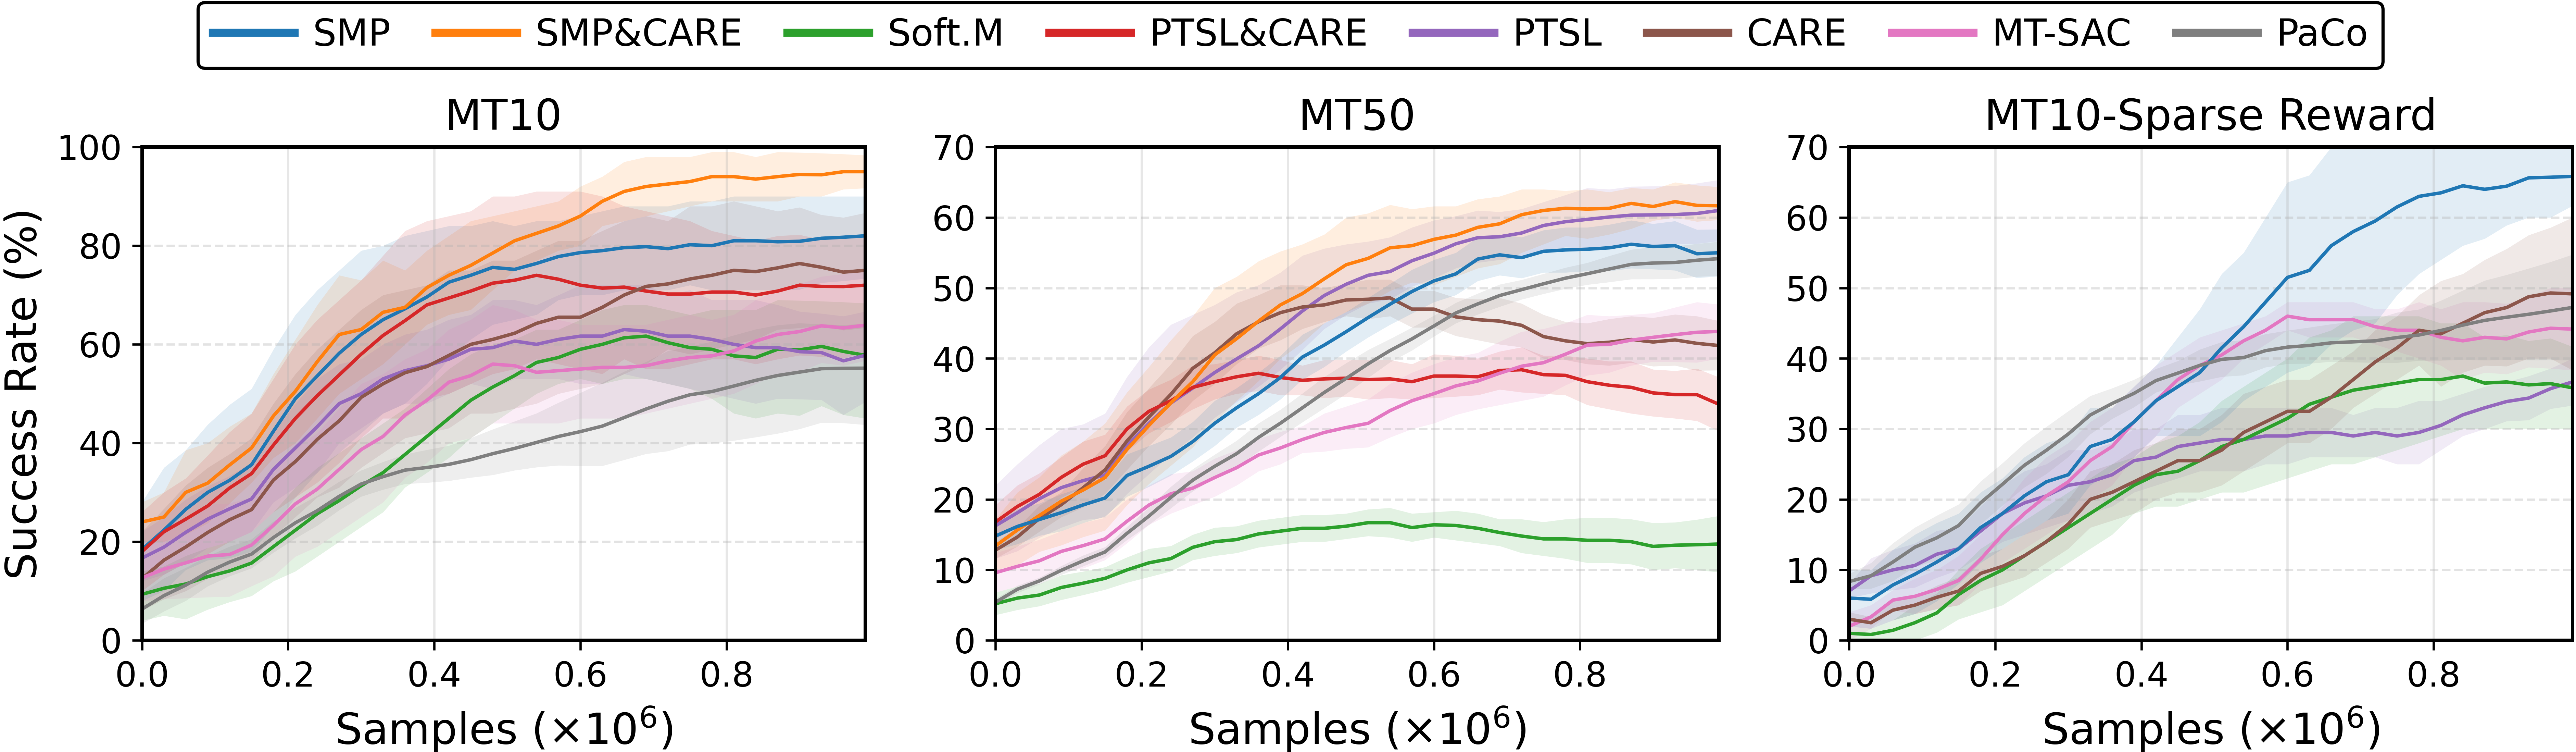
\includegraphics[width=14.4cm,height=4cm]{L-8.png}\\
\caption{Comparison of SMP against baselines on one benchmark setting.}
\label{fig:fig_l}
\end{figure*}

As illustrated in Fig.~\ref{fig:fig_l}, SMP consistently achieves the highest average success rate and the fastest convergence across all evaluated methods. We attribute this performance gain to the stage-aware modular design, which enables efficient knowledge reuse and reduces negative interference between task stages.

For a fair comparison, all models are implemented with comparable network architectures and hyperparameters (Appendix~B). 
Table~\ref{table:m} reports the success rates under three model sizes. Notably, when combined with CARE, SMP achieves a peak accuracy of 95.0\%. 
These results demonstrate both the compactness and the compositional synergy enabled by our approach.

We further assess training stability. 
As shown in Table~\ref{table:s}, SMP yields the lowest standard deviation and highest minimum score, indicating robust convergence. 
This improvement is mainly attributed to mask-based stage policy activation, which effectively reduces interference between tasks and leads to more stable training.



\begin{table}[htbp]
  \centering
  \begin{tabular}{c cc ccc}
    \toprule
    \multirow{2}{*}{\textbf{Methods}} & 
    \multicolumn{2}{c}{\textbf{MT-10(\%)}} & 
    \multicolumn{2}{c}{\textbf{MT-50(\%)}} \\
    \cmidrule(lr){2-3} \cmidrule(lr){4-5}
    &  \textbf{Mean} & \textbf{SD} & 
     \textbf{Mean} & \textbf{SD} \\
    \midrule
    MT-SAC          & 44.1 & -  & 35.0 & - \\
    Soft.M          & 35.8  & -  & 13.1  & -   \\
    CARE            & 49.1  & -  & 20.6 & - \\
    PTSL            & 36.6  & -  & 27.6  & -   \\
    PTSL\&CARE      & 56.6  & -  & 35.3  & - \\
    PaCo            & 47.2  & -    & 7.6   & -   \\
    \midrule
    \textbf{SMP (Ours)}     & \textbf{62.5} & - & \textbf{39.5}  & -  \\
    \textbf{SMP\&CARE}       & - & - & -  & - \\
    \bottomrule
  \end{tabular}
    \caption{Success rate (\%) comparison on MT-10 and MT-50 with \textbf{Sparse} rewards.}
      \label{table:s}
\end{table}

\begin{table}[htbp]
  \centering
  \begin{tabular}{c cc ccc}
    \toprule
    \multirow{2}{*}{\textbf{Methods}} & 
    \multicolumn{2}{c}{\textbf{MT-10(\%)}} & 
    \multicolumn{2}{c}{\textbf{MT-50(\%)}} \\
    \cmidrule(lr){2-3} \cmidrule(lr){4-5}
    &  \textbf{Mean} & \textbf{SD} & 
     \textbf{Mean} & \textbf{SD} \\
    \midrule
    MT-SAC          & 63.8 & 4.7  & 43.4 & 2.5 \\
    Soft.M          & 53.8  & 9.0  & 13.6  & 4.0   \\
    CARE            & 77.0  & 7.1  & 45.3 & 2.8 \\
    PTSL            & 60.4 & 6.1  & 61.6  & 6.6   \\
    PTSL\&CARE      & 74.4  & 4.1  & 33.4  & 3.1 \\
    PaCo            & 56.8  & 10.1    & 54.4   & 5.7   \\
    \midrule
    \textbf{SMP (Ours)}     & \textbf{81.2} & \textbf{3.2} & 55.0  & \textbf{2.1}  \\
    \textbf{SMP\&CARE}       & \textbf{93.3} & \textbf{1.6} & \textbf{62.2}  & 7.7 \\
    \bottomrule
  \end{tabular}
    \caption{Success rate (\%) comparison on MT-10 and MT-50 with \textbf{Dense} rewards.}
      \label{table:d}
\end{table}



We further evaluate SMP’s few-shot adaptability scenarios; results and analysis are detailed in Appendix.B

\paragraph{Sparse Reward.}

To assess robustness under minimal supervision, we evaluate all methods in a sparse reward setting, where agents receive $r = -1$ at every step unless a task is completed ($\sigma^{(i)}_{n}(s)=1$). This simulates realistic scenarios where dense reward is unavailable.


As shown in Table~\ref{table:s}, most baselines perform poorly due to vanishing gradients and insufficient exploration. 
In contrast, SMP achieves a $62.5\%$ success rate, significantly higher than all baselines. 
We attribute this improvement to two key mechanisms in our framework: (1) the stage reward, which provides intermediate intrinsic feedback at stage transitions, thereby alleviating sparse supervision and improving credit assignment; and (2) the stage-masked policy, which enables finer-grained action control through stage-specific policies.
These mechanisms work in concert to enable stable and efficient learning in sparse-reward multitask settings. We further analyze their individual and combined contributions through targeted ablation studies in Section~5.3.





\subsection{Ablation Studies}

First, we perform an ablation experiment on the frequency parameter $B$ governing the use of SMP. 
In our design, the evaluation interval $B$ governs multiple functionalities simultaneously: (1) the mask update and pruning/regrowth cycles, (2) cross-stage similarity calculation, and (3) obtaining high-return action subsequences within a certain interval.  
Table~\ref{tab:eval_interval} reports performance under different evaluation intervals. 

The results clearly indicate that reducing the usage frequency of SMP leads to a degradation in performance. 
Specifically, as the evaluation interval $B$ increases from 4500 to 27000, the final success rate drops from 78.3\% to 70.0\%. 
This suggests that structural adaptation and behavior alignment are crucial for effective transfer in MTRL settings. When SMP is deactivated entirely ($B \to \infty$), performance drops further to match that of the MT-SAC baseline.


\begin{table}[htbp]
\centering

\begin{threeparttable}
\begin{tabular}{lc}
\toprule
\textbf{Evaluation Interval (steps)} & \textbf{Success Rate (\%)} \\
\midrule
4500 & 78.3 \\
9000 & 76.7 \\
18000 & 71.6 \\
27000 & 70.0 \\
\bottomrule
\end{tabular}
\caption{Impact of Evaluation Interval on SMP Performance (MT-10)}
\label{tab:eval_interval}
\begin{tablenotes}[flushleft]
\footnotesize
\item All results are reported for random seed 1 under identical training and architecture settings.
\end{tablenotes}
\end{threeparttable}
\end{table}



We next disentangle the individual contributions of the stage reward and the stage-masked policy in the sparse reward regime (Table~\ref{tab:sparse}).
Starting from the MT-SAC (41.6\%), adding the intrinsic stage reward (Section 3) improves performance to 58.3\%, validating the benefit of stage reward. 
Applying the stage-masked policy alone also leads to an improvement (56.7\%), indicating the utility of fine-grained policy modulation. 
Notably, combining both mechanisms in the full SMP yields the highest performance (68.3\%), underscoring their complementary benefits.

\begin{table}[htbp]
\centering
\begin{threeparttable}
\begin{tabular}{lc}
\toprule
\textbf{Methods} & \textbf{Success Rate (\%)} \\
\midrule
\text{SAC} & 41.6 \\
\text{$+$Stage reward} & 58.3 \\
\text{$+$Stage-Masked Policy} & 56.7 \\
\text{SMP} & 68.3 \\
\bottomrule
\end{tabular}
\caption{Stage Rewards \& Stage Policies (MT-10)}
\label{tab:sparse}
\begin{tablenotes}[flushleft]
\footnotesize
\item The table experiments are all sparse reward settings, and the random seeds are all set to 1.
\end{tablenotes}
\end{threeparttable}
\end{table}



Additional ablations on stage segmentation and similarity design (Appendix~B) further validate that fine-grained task structure and behavior-driven alignment enhance SMP’s effectiveness.


\section{Conclusion}

This paper introduces the concept of task stages to enable more flexible and effective cross-task knowledge transfer in MTRL. 
We propose the SMP framework, which leverages a TCN-based similarity function to align sub-task behaviors across different stages and adopts a mask-based policy mechanism for stage-centered policy activation and reuse. 
Comprehensive experiments demonstrate that SMP substantially improves both performance and robustness in structured MTRL benchmarks, especially under sparse reward conditions, outperforming several strong baselines.

A limitation is reliance on tasks with explicit stage-wise structure, which may restrict applicability. 
Future work will extend SMP to infer task stages or adapt to less-structured environments, broadening its generality and impact.




\appendix

\section*{Ethical Statement}

There are no ethical issues.

\section*{Acknowledgments}

The preparation of these instructions and the \LaTeX{} and Bib\TeX{}
files that implement them was supported by Schlumberger Palo Alto
Research, AT\&T Bell Laboratories, and Morgan Kaufmann Publishers.
Preparation of the Microsoft Word file was supported by IJCAI.  An
early version of this document was created by Shirley Jowell and Peter
F. Patel-Schneider.  It was subsequently modified by Jennifer
Ballentine, Thomas Dean, Bernhard Nebel, Daniel Pagenstecher,
Kurt Steinkraus, Toby Walsh, Carles Sierra, Marc Pujol-Gonzalez,
Francisco Cruz-Mencia and Edith Elkind.


%% The file named.bst is a bibliography style file for BibTeX 0.99c
\bibliographystyle{named}
\bibliography{ijcai26}

\end{document}

